\section{Study Design and Data Collection}
\label{sec:study-design}
We crafted two studies to understand the decision making factors and reasoning patterns of a diverse population regarding AI use cases. In this section, we discuss the selection of use cases (\S~\ref{ssec:use-cases}), survey designs for the two studies (\S~\ref{ssec:survey-design}) and data collection details and participant demographics (\S~\ref{ssec:data-and-demographics}).


\subsection{Use Cases}
\label{ssec:use-cases}
We define an AI use case as one where an AI system replaces a specific role or function, and we follow three of the five concepts used in EU AI Act to describe each use case \citep{golpayegani2023risk}: the domain, purpose, and capabilities. To understand how different characteristics of an AI use case can impact judgments and decision making processes, we first chose two broad areas of AI involvement that were frequently brought up by the public when discussing use cases in AI \citep{kieslich2024myfuture,mun2024participaidemocraticsurveyingframework}: AI in personal, everyday usage and AI in labor replacement. Additionally, these two areas of focus were chosen as they were easy for participants to fully comprehend an AI system taking on the role (e.g., AI lawyer) compared to other use cases (e.g., AI for climate change). We then crafted five use cases per category by varying EU AI risk level for the personal use cases and required entry level education for the labor replacement use cases. While we explored multiple domains for labor replacement use cases, we chose to focus on the personal health domain for personal use cases, reflecting the public's interest \citep{mun2024participaidemocraticsurveyingframework,kieslich2024myfuture}. In the use case descriptions, we focus on text-based, non-embodied, digital systems, to ensure that an AI system can fully replace the role/function online.

\subsection{Use Cases Specialization}\label{sec:usecase}

\begin{figure}
    \centering    
{\footnotesize
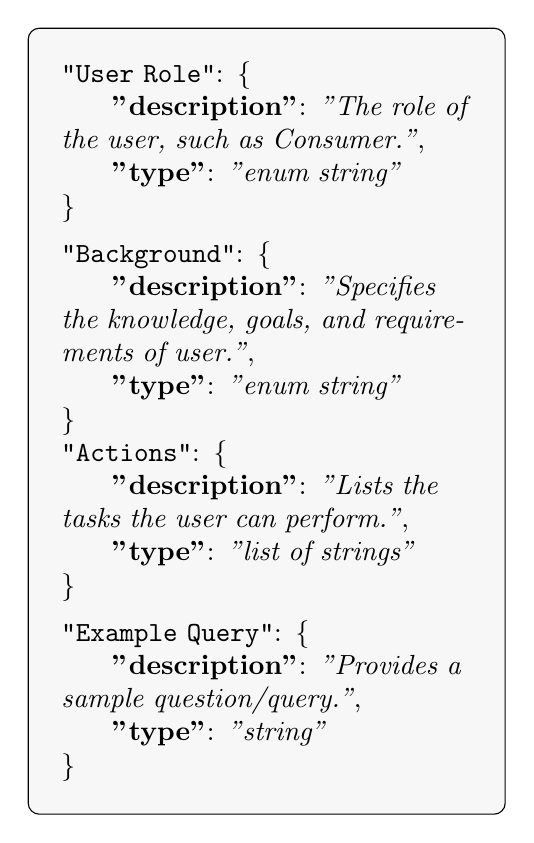
\begin{tikzpicture}
% Draw rounded rectangle with shadow
\node[rectangle, rounded corners, draw=black, fill=black!3!white, text width=0.43\textwidth, inner sep=12pt, align=left] (box) {
    \textbf{\texttt{"User Role"}}: \{\\
    \hspace{15pt} \textbf{"description"}: \textit{"The role of the user, such as Consumer."}, \\
    \hspace{15pt} \textbf{"type"}: \textit{"enum string"} \\
    \} \vspace{5pt}\\
    \textbf{\texttt{"Background"}}: \{\\
    \hspace{15pt} \textbf{"description"}: \textit{"Specifies the knowledge, goals, and requirements of user."}, \\
    \hspace{15pt} \textbf{"type"}: \textit{"enum string"} \\
    \} \\
    \textbf{\texttt{"Actions"}}: \{\\
    \hspace{15pt} \textbf{"description"}: \textit{"Lists the tasks the user can perform."}, \\
    \hspace{15pt} \textbf{"type"}: \textit{"list of strings"} \\
    \} \vspace{5pt}\\
    \textbf{\texttt{"Example Query"}}: \{\\
    \hspace{15pt} \textbf{"description"}: \textit{"Provides a sample question/query."}, \\
    \hspace{15pt} \textbf{"type"}: \textit{"string"} \\
    \}
};

\end{tikzpicture}
}
\caption{Use case specializations. For each use case, we define its role, goal, actions, and example query. For each property, we present its description and type.}
\label{fig:usecasedef}
\end{figure}

\begin{table*}[]
\centering
\caption{The actions and example query for each kind of user role defined for \chatiot.}
\label{tab:usecase}
\resizebox{\textwidth}{!}{

\begin{tabular}{p{1.5cm}|p{12cm}|p{4cm}}
%\begin{tabular}{@{}c@{\hskip 0.1cm}|
%    @{\hskip 0.1cm}>{\arraybackslash}p{10.5cm}@{\hskip 0.1cm}|
%    @{\hskip 0.1cm}>{\arraybackslash}p{5cm}@{\hskip 0.1cm}
%    }
\toprule
\toprule
\multicolumn{1}{c|}{Role} & \multicolumn{1}{c|}{Actions} & \multicolumn{1}{c}{Example Query}  \\ \midrule
Consumer  
& \romannumeral1) Assess the security of IoT devices before purchase or installation; \newline
\romannumeral2) Monitor ongoing security status and updates for existing devices;\newline
\romannumeral3) Make informed decisions based on security reports provided by \chatiot.
& Is it secure to use Signify Smart Lighting in home? \\
\midrule

Security Analyst  
&
\romannumeral1) Identify and evaluate security threats and vulnerabilities in IoT devices;\newline
\romannumeral2) Recommend mitigation strategies based on threat intelligence and analysis;\newline
\romannumeral3) Provide detailed security reports to stakeholders.
& Conduct a security assessment for TP-Link AX6000 Wi-Fi 6 Router. 
\\ \midrule

Technical Officer 
&
\romannumeral1) Ensure that IoT devices are deployed securely and operate within compliance guidelines;\newline
\romannumeral2) Oversee the application of security updates and patches;\newline
\romannumeral3) Monitor the security posture of the IoT ecosystem within their organization.
& Check the security labeling of the company's WiFi Routers,  including TP-Link, D-Link, and ASUS in Singapore. 
\\
\midrule

Developer
&
\romannumeral1) Design and develop secure IoT products by adhering to best practices and security standards;\newline
\romannumeral2) Continuously update products to address new vulnerabilities and threats;\newline
\romannumeral3) Provide accurate security documentation and updates to customers.
&
Develop a security enhancement roadmap for the next generation of TP-Link Wi-Fi routers.
\\
\midrule

Trainer 
&
\romannumeral1) Develop and deliver training programs on IoT security;\newline
\romannumeral2) Guide users and organizations on how to secure IoT devices and respond to incidents;\newline
\romannumeral3) Provide up-to-date information on IoT security trends and best practices.
&
Prepare a guide on the importance of cybersecurity labeling for smart locks like the August Smart Lock.
\\
\bottomrule
\bottomrule

\end{tabular}}
\end{table*}

In this section, we define five specialized use cases of \chatiot. 
Each use case is defined by \textit{four} fundamental properties: \textit{User Role}, \textit{Background}, \textit{Actions}, and \textit{Example Query}, within the IoT security domain.
The detailed specifications are illustrated in Figure~\ref{fig:usecasedef}.
The roles include \textit{Consumer}, \textit{Security Analyst}, \textit{Technical Officer}, \textit{Developer}, and \textit{Trainer}. 
Recall that we have discussed background in \S~\ref{sec:resgen}, we present the detailed actions and example query in the following context.


Table~\ref{tab:usecase} highlights the key actions associated with each user role, such as assessing the security of IoT devices, deploying security patches, or developing training programs on IoT security.
Additionally, it provides example queries for each role, demonstrating how \chatiot\ can be utilized to address the unique needs of various users. 
This structured approach ensures that \chatiot\ caters to a diverse range of users, offering tailored assistance and enhancing IoT security management across different scenarios.
Note that while we provide five use cases, they are not rigid or fixed. 
The use cases can be easily extended by defining new user roles, specifying the background (including knowledge, goals, and requirements), and outlining actions. Example queries can also be added to further clarify the context and functionality of each user role.


\paragraph{Labor Replacement Use Case Scenarios} 
For the first area of focus, AI in labor replacement, we collect jobs listed in the U.S. census bureau\footnote{} and sort them according to entry level education required as stated in the census. Education level has been tightly linked to socioeconomic status \citep{} and occupational status \citep{}, which signals the level of expertise and trust \citep{svensson2006professional,evetts2006introduction}. We select jobs that have a large portion of digital or intellectual components with minimal requirement for embodiment. We select the following five labor roles: Lawyer, Elementary school teacher, IT support specialist, Government support eligibility interviewer, and Telemarketer. See Table~\ref{tab:use-cases} for further details.

\paragraph{Personal Use Case Scenarios} 
 To comprehensively understand the acceptability of different applications in personal and private life, we varied the risk levels in the use cases following the EU AI Act to high risk, high / limited, limited, limited / low, and low risk. Furthermore, to confirm that the AI risk levels were reflected in the description, we ensured that the categories assigned by GPT-4 following \citeauthor{herdel2024exploregen} agreed with the research team's assignment. For these use cases, we adapted the descriptions of the systems written by participants from prior works \citep{mun2024participaidemocraticsurveyingframework,kieslich2024myfuture}. See Table~\ref{tab:use-cases} for further details.


\subsection{Survey Design}
\label{ssec:survey-design}
\subsubsection{Overview}
To understand how people make judgments about AI use cases, we designed two studies that collect acceptability and usage judgments, which were administered to two separate groups of participants. In both studies, we ask participants to make judgments on 1) whether the use case should exist or not and 2) whether the participant would use the application if it existed. However, the two studies differ in their elicitation of the participant's reasoning process. 

\paragraph{Study 1: Perception of Five AI Use Cases}
To understand the unprompted, immediate reasoning process of participants, the first study collects use case judgments without further guidance by showing participants five different use case descriptions from one of the use case scenarios from \S~\ref{ssec:use-cases}. After reading a brief description of each use case, the participants are asked to choose whether the application should be developed or not. The reasoning process is collected through an open text question that asks participants to 1) elaborate on their decisions and 2) provide a condition in which they would switch the decision. Thus, the first question asks about the main reasons for their decision and the second question elicits the primary concern when considering the counterfactual decision. 
% We repeat the same sets for 5 different use cases for each participant to account for the variability in the individuals and to assess the use case factors in judgment within subjects as well as between subjects (RQ4; Q\#).  

\paragraph{Study 2: Guided Weighing of a Single Use Case}
To understand the impact to the decision making process of participants when specifically asked to weigh the possible harms and benefits of a use case (\reasoningeffect), the second study utilizes the framework developed by \citet{mun2024participaidemocraticsurveyingframework}, which contains a comprehensive set of questions to ask participants about positive and negative impacts of use case development as well as the impacts of not developing the application. In our survey, we show participants a single, pre-determined use case drawn from the same set of use cases from the first study. While we collect judgments both before and after the explicit harms and benefits consideration, after the questions about harms and benefits, we ask participants to elaborate on their decisions and to specify the conditions (if any) for them to switch their decisions.

\subsubsection{Survey Questions}
\label{sssec:survey-qs}
In both surveys, we ask participants to read one or more descriptions of AI use cases and to make two judgments: 1) ``Do you think a technology like this should exist?'' (Q1) and 2) ``If the <\textit{use case}> exists, would you use its services?'' (Q5). A question to indicate their level of confidence is asked following each question (Q2, Q6). As discussed above, the two surveys differ in eliciting reasoning. The participants are asked to both elaborate on their decisions (Q3) and specify the conditions under which they would switch their decisions (Q4). While these same set of questions are asked for all five use cases for Study 1, in Study 2, we further ask participants to weigh the harms and benefits of the use case in the context of both developing and not developing it. We then again ask participants the same set of judgment questions (Q1-2, Q5-6) along with the same open-text questions to elaborate on their reasoning (Q3, Q4).

\paragraph{Harms and Benefits (Study 2)} 
To gather explicit weighing of harms and benefits of a use case, we ask participants to write in free-text the positive and negative impacts, the groups that would be harmed or benefited the most, and the scale of such impacts. We repeat this process for both scenarios of developing and not developing the use case. To minimize the ordering effect, we randomize the order in which participants answer questions about the scenarios, developing and not developing, harms and benefits, and the types of harms of developing (functionality error or misuse).

\paragraph{AI Literacy and Demographics}
Following the main survey, we asked participants questions about their AI literacy and demographics, to explore both the demographic factors and AI literacy that affect decision making of use cases (\demofactor). In the AI literacy section of the survey, we asked participants to indicate their familiarity with AI in awareness, usage, evaluation, and ethics as well as frequency of AI usage and knowledge of their shortcomings \citep{wang2023measuring,mun2024participaidemocraticsurveyingframework}. In addition to the demographic information of the participants such as race, sex, age, employment status, income, and level of education, we also collected information about their discrimination experiences \citep{kingsley2024investigating}. 

\paragraph{Questionnaires}
To further understand the decision making styles of participants that could inform AI use case decision making (\reasoningfactor), we adopted three questionnaires in our survey: Moral foundations questionnaire \citep{graham2008moral}, Oxford Utilitarianism Scale \citep{kahane2018beyond}, and Toronto empathy questionnaire \citep{spreng2009toronto}. These questionnaires were included at the end of the survey so as not to influence the decisions of the participants in the main portion of the survey. 

\subsection{Data Collection and Participant Demographics}
\label{ssec:data-and-demographics}
We used Prolific\footnote{} to recruit participants. To represent diverse sample, we stratified our recruitment by the ethnicity categories (White, Mixed, Asian, Black and Other) and age (18-48, 49-100) provided by Prolific. We also added criteria for quality such as survey approval rating, previous number of surveys, etc. Our study was approved by IRB at our institutions, and we paid 12 USD/hour, adjusting post-hoc for older age group, which took longer time to complete the surveys. After filtering the survey responses, our final sample consisted of 398 participants across 4 surveys, with the age and race of the participants shown in \input{tables/demographic-data/short-demographics} and the distribution of each use case for Study 2 in \begin{table}[!hbpt]
    \centering
    \small
    \begin{tabularx}{0.4\linewidth}{l|X}
    \toprule
       Use Case & Participants Allocated \\
    \midrule
       Personal Use Cases & \\
    \midrule
       Digital Medical Advice & 20 \\
       Customized Lifestyle Coach & 20 \\
       Personal Health Research & 19 \\
       Nutrition Optimizer & 21 \\
       Flavorful Swaps & 17 \\
    \midrule
       Labor Replacement Use Cases & \\
    \midrule
       Lawyer & 20 \\
       Elementary School Teacher & 22 \\
       IT Support Specialist & 17 \\
       Government Eligibility Interviewer & 19 \\
       Telemarketer & 23 \\
    \bottomrule
    \end{tabularx}
    \caption{Use Case allocation for Study 2. Specific participant numbers are listed for each use case.}
    \label{tab:study2-use-case}
\end{table}.